\chapter{Tái tạo kết quả thí nghiệm Convolutional Neural Network}
\label{Appendix2}

Ngoài việc tìm bộ siêu tham số cho kết quả tốt nhất, chúng tôi cũng cố gắng tái tạo kết quả mà bài báo đã công bố. Chúng tôi thực hiện quá trình tái tạo này để kiểm tra tính khả thi của các kết quả mà bài báo đã công bố. Hình \ref{fig:exp-cnn-rep} là kết quả sát nhất với bài báo mà chúng tôi có thể tái tạo được từ khoảng tìm kiếm mà chúng tôi sử dụng. Có thể thấy được rằng, đường đi của các thuật toán trong hình \ref{fig:exp-cnn-best}a và \ref{fig:exp-cnn-rep} có dạng khá giống nhau. Mặc dù có thể tái tạo được hình dạng biểu đồ của các thuật toán, độ lỗi cuối cùng của các thuật toán trong hình \ref{fig:exp-cnn-rep} vẫn cao hơn so với kết quả tốt nhất mà chúng tôi ghi nhận được ở hình \ref{fig:exp-cnn-best}b.

\begin{figure}[htp]
	\centering
	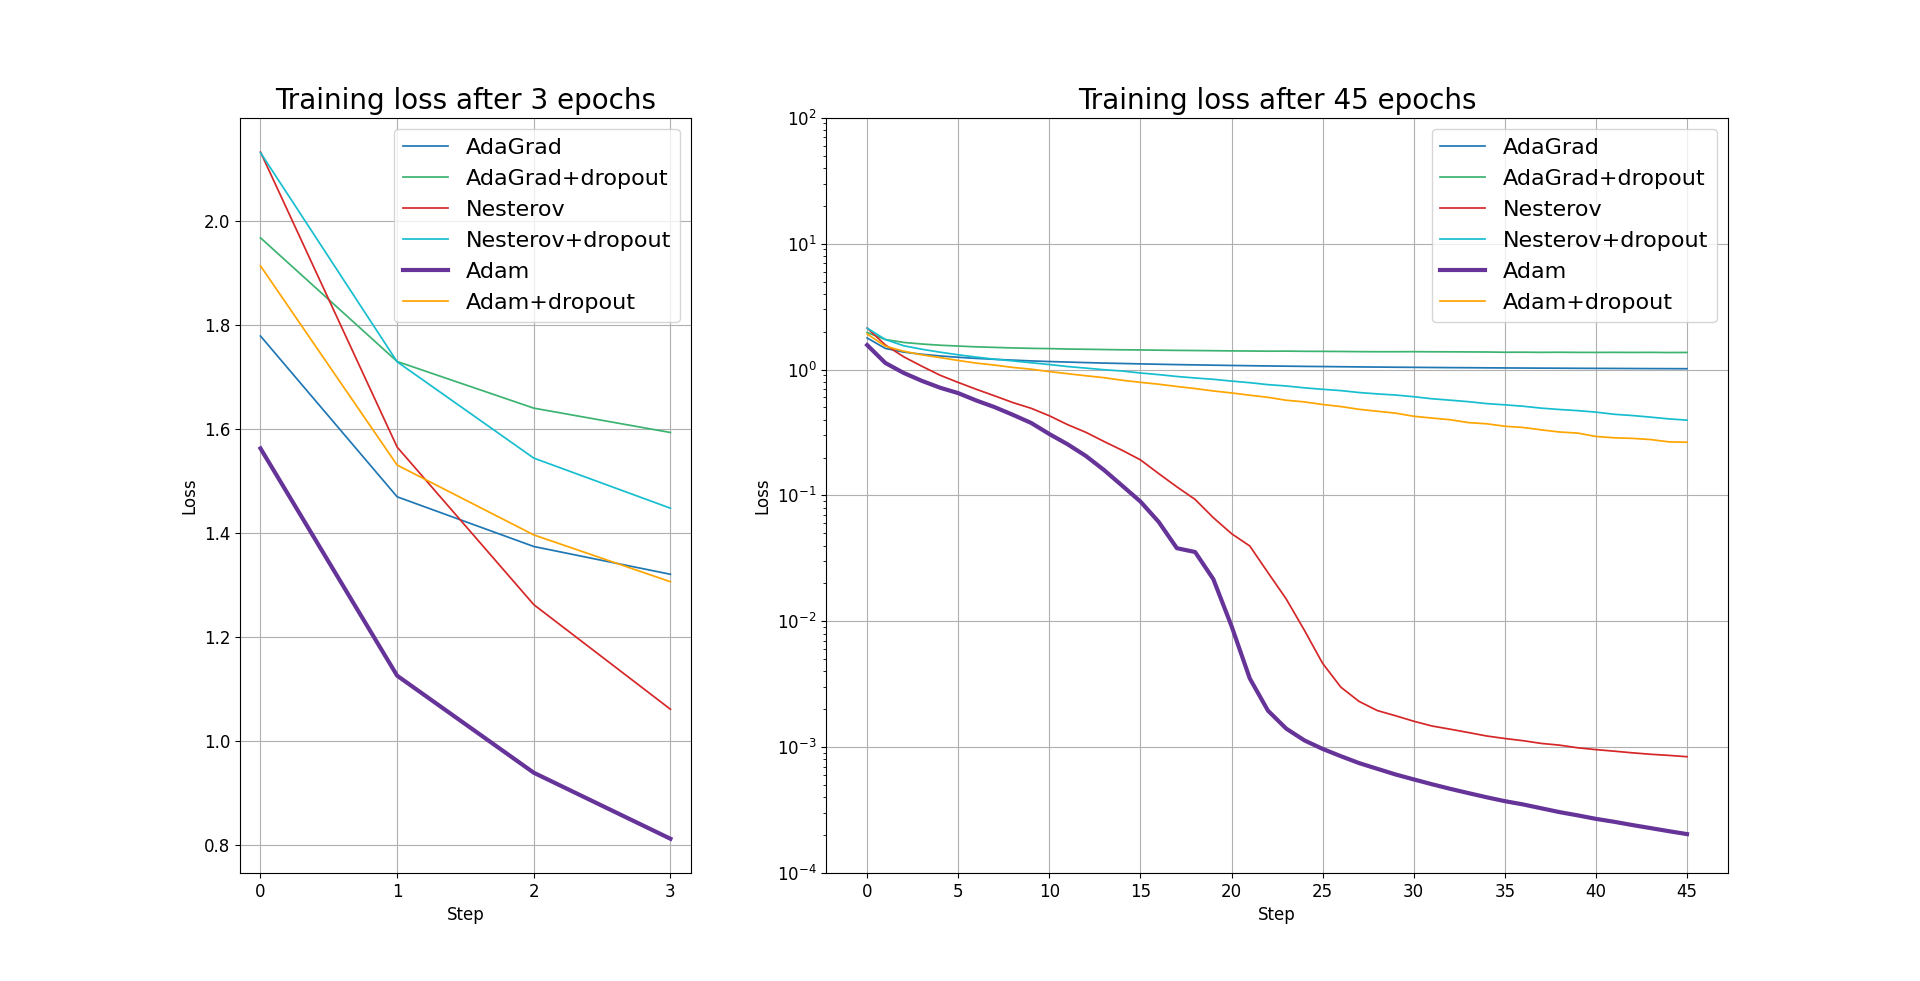
\includegraphics[width=140 mm]{images/cnn-rep.png}
	\caption{Kết quả thí nghiệm Convolutional Neural Network giữa thuật toán mà chúng tôi cài đặt với bộ siêu tham số mô phỏng kết quả của bài báo.}
	\label{fig:exp-cnn-rep}
\end{figure}

Ngoài lí do tác giả không công bố siêu tham số, cũng như tính chất ngẫu nhiên của SGD, một nguyên nhân khả thi khác cho sự khác biệt giữa kết quả mà chúng tôi ghi nhận được so với kết quả mà bài báo công bố là bản chất cài đặt của thư viện. Mỗi thư viện có cách xử lý tính toán riêng dẫn đến kết quả có phần lệch nhau. Vì tác giả cũng không nói rõ thư viện được sử dụng trong bài báo, nên thư viện Pytorch mà chúng tôi sử dụng có thể sẽ ra kết quả khác so với bài báo.